\chapter{Quantum Entanglements, Part 1}

These notes follow Leonard Susskind's seventh lecture on quantum entanglement, curated by LazyingArt LLC. The lecture begins in repair mode. Susskind does not yet launch into entanglement entropy; instead he goes back and finishes the two-slit discussion in the simplest possible discrete language. That is the right starting point, because the real issue is not the geometry of the slits but the fate of interference once some apparatus records which route the electron took. Only after that mechanism is made precise does he turn to entropy, trace, and density matrices, which are the tools he will need next time.

\section{Finishing the Discrete Two-Slit Setup}

We begin with a stripped-down model. There is a source at a site labeled \(0\), two openings labeled \(A\) and \(B\), and a screen whose possible arrival sites are denoted by \(|m\rangle\). Everything else in the barrier is regarded as blocked off. For the moment the electron's own spin is irrelevant and is set aside; the states are characterized only by position.

The governing principle is linearity. If a state begins as a linear combination, then under time evolution it becomes the corresponding linear combination of the separately evolved pieces. In the symmetric situation Susskind writes, schematically,
\begin{equation}
|0\rangle \longrightarrow |A\rangle + |B\rangle .
\end{equation}
This line is deliberately schematic. The lecture suppresses normalization on the board. A fully normalized version would carry an overall factor of \(1/\sqrt{2}\), but that factor is not the point here; the point is that the source feeds both slits with equal amplitude.

Once the electron reaches one slit or the other, it propagates to the screen. The two route amplitudes are written
\begin{align}
|A\rangle &\longrightarrow \sum_m \psi_m |m\rangle , \\
|B\rangle &\longrightarrow \sum_m \phi_m |m\rangle .
\end{align}
Here \(\psi_m\) is the amplitude for an electron that started at \(A\) to arrive at the \(m\)-th site on the screen, and \(\phi_m\) is the corresponding amplitude from \(B\).

\begin{figure}[h]
\centering

\includegraphics[width=0.72\textwidth]{lecture_07_figure_02.png}
\caption{Lecture board: screen-basis amplitude expansion.}
\end{figure}

The lecture insists on the order of construction. First we understand the propagation from \(A\) alone and from \(B\) alone. Only then do we reopen both holes and ask what quantum mechanics really says.

\section{From Path Amplitudes to the Interference Term}

Suppose first that hole \(B\) is closed. Then the amplitude to arrive at site \(m\) is simply \(\psi_m\), so the probability is
\begin{equation}
P_A(m)=\psi_m^*\psi_m .
\end{equation}
If instead hole \(A\) is closed and only \(B\) is open, then
\begin{equation}
P_B(m)=\phi_m^*\phi_m .
\end{equation}

At this point classical instinct suggests the wrong answer. One is tempted to say that if both holes are open, then the probability at \(m\) should be the sum of these two probabilities. Susskind pauses here to mark the pivot: not so in quantum mechanics. What we add are amplitudes.

With both slits open, linearity gives
\begin{equation}
|A\rangle+|B\rangle \longrightarrow \sum_n (\psi_n+\phi_n)|n\rangle .
\end{equation}
So at a fixed screen site \(m\), the relevant amplitude is \(\psi_m+\phi_m\). The probability is therefore
\begin{align}
P_m &= |\psi_m+\phi_m|^2 \\
&= \psi_m^*\psi_m+\phi_m^*\phi_m+\psi_m^*\phi_m+\phi_m^*\psi_m .
\end{align}
The first two terms are the direct route contributions. The last two are the interference terms. They are the genuinely quantum part of the story.

The lecture then dramatizes this with the simplest symmetry arguments. At the symmetry point on the screen we expect
\begin{equation}
\psi_m=\phi_m ,
\end{equation}
and then the probability is enhanced. In the lecture's shorthand one gets four times the single-route contribution. On the other hand, if the geometry and phases are such that
\begin{equation}
\psi_m=-\phi_m ,
\end{equation}
then the amplitudes cancel and
\begin{equation}
P_m=0 .
\end{equation}
So despite the fact that the electron can get to \(m\) through \(A\) and it can get to \(m\) through \(B\), with both slits open it may fail to arrive there altogether. That is the weirdness Susskind wants sitting in plain view before he asks the next question.

\begin{figure}[h]
\centering

\includegraphics[width=0.74\textwidth]{lecture_07_figure_03.png}
\caption{Lecture board: interference probability and cross terms.}
\end{figure}

Now the lecture can make the real turn: what happens if the experiment is arranged so that the route is recorded?

\section{Which-Path Recording as Entanglement with a Spin}

Susskind introduces the simplest recording apparatus he can think of: an auxiliary spin with two states, \(u\) and \(d\). This could in principle be the electron's own spin, but he explicitly asks us not to think of it that way. The point is to model an external detector, however simple, that can register passage through one slit and not the other.

The initial state is therefore not just the electron at the source. It is the electron at the source together with the detector in its untriggered state:
\begin{equation}
|0,d\rangle .
\end{equation}
The rules of the model are simple. If the electron passes through slit \(A\), it flips the detector from down to up. If it passes through \(B\), the detector remains down. So the post-slit state is
\begin{equation}
|0,d\rangle \longrightarrow |A,u\rangle + |B,d\rangle .
\end{equation}
From there the electron propagates to the screen just as before, except that the detector state comes along as a route label:
\begin{align}
|A,u\rangle &\longrightarrow \sum_n \psi_n |n,u\rangle , \\
|B,d\rangle &\longrightarrow \sum_n \phi_n |n,d\rangle .
\end{align}
The final state is thus
\begin{equation}
|\Psi_{\mathrm{final}}\rangle
=
\sum_n \bigl(\psi_n|n,u\rangle+\phi_n|n,d\rangle\bigr) .
\end{equation}

The important change is now visible. We do not have a single electron wave function over the screen. We have a superposition of two branches, and each branch carries a different detector record.

\subsection{Question \& Answer}

\paragraph{Question.} Did the wave packet collapse, or did the electron become entangled with the detector?

\paragraph{Answer.} Susskind's answer is that both ways of speaking occur, but they are not equally sharp. If we insist on describing only the electron and forgetting the detector, then one may use the old language of collapse: the interference terms are gone, and one says the wave packet has collapsed to one route or the other. But if we include the apparatus in the description, then that is not what has happened. The composite system has not become only one branch. It has become
\[
|A,u\rangle + |B,d\rangle ,
\]
an entangled state of electron and detector. In that fuller description the correct statement is not ``collapse occurred'' but ``entanglement was established.''

This correction matters because the lecture is trying to replace vague talk of measurement with a precise mechanism. If we keep the apparatus in view, we can see exactly where the interference goes.

\section{Projector onto a Screen Position and Loss of Cross Terms}

Having set up the entangled state, Susskind deliberately slows down and does the formal calculation. We want the probability that the electron is found at a particular screen site \(m\).

In the enlarged Hilbert space, the property ``the electron is at \(m\)'' defines a two-dimensional subspace. The basis states of that subspace are
\[
|m,u\rangle
\qquad \text{and} \qquad
|m,d\rangle .
\]
Therefore the projector onto that subspace is
\begin{equation}
\Pi_m = |m,u\rangle\langle m,u| + |m,d\rangle\langle m,d| .
\end{equation}
This is exactly the object the board snapshot preserves most clearly.

\begin{figure}[h]
\centering

\includegraphics[width=0.68\textwidth]{lecture_07_figure_04.png}
\caption{Lecture board: projector onto a fixed screen position.}
\end{figure}

The probability of arrival at \(m\) is the expectation value of this projector in the final state:
\begin{equation}
P_m=\langle \Psi_{\mathrm{final}}|\Pi_m|\Psi_{\mathrm{final}}\rangle .
\end{equation}
Substituting the final state gives
\begin{align}
P_m
&=
\sum_{n,n'}
\bigl(\psi_n^*\langle n,u|+\phi_n^*\langle n,d|\bigr)
\Pi_m
\bigl(\psi_{n'}|n',u\rangle+\phi_{n'}|n',d\rangle\bigr) .
\end{align}
Now one sees why Susskind kept saying that \(\psi_m\) and \(\phi_m\) multiply different ket vectors. The projector can pair \(|n,u\rangle\) only with \(|m,u\rangle\), and \(|n,d\rangle\) only with \(|m,d\rangle\). In particular,
\begin{equation}
\langle u|d\rangle=0 .
\end{equation}
So the mixed terms vanish. The only surviving contributions are the direct ones, with matching screen label and matching detector label. Hence
\begin{equation}
P_m = |\psi_m|^2 + |\phi_m|^2 .
\end{equation}

This is the formal centerpiece of the lecture. The interference terms do not disappear because we announced a collapse postulate. They disappear because a measurement has correlated the route alternatives with orthogonal detector states. One must match not only the endpoint on the screen, but also the detector label. Once that extra label is there, the two amplitudes no longer add into a single coherent amplitude at \(m\).

\section{What Counts as a Measurement?}

Once the clean spin model is on the board, the lecture opens out into a long Socratic clarification. The point is not to leave the spin as an artificial toy. It is to identify the general rule behind it.

The rule is this: a measurement has occurred if some mark has been left on the world from which one can, in principle, infer which alternative took place. No conscious observer is required at that stage. A human being may later read the record, but the decisive event is that the record exists.

\subsection{Question \& Answer}

\paragraph{Question.} What counts as a measurement?

\paragraph{Answer.} Any interaction that leaves a distinguishable route record counts as a measurement. If the record states are orthogonal, interference is destroyed completely. If they overlap, the interference is only partially washed out.

The lecture first tests the symmetric placement of the detector. Suppose the auxiliary spin is placed so that it is kicked in exactly the same way whether the electron passes through \(A\) or through \(B\). Then the record state is the same on both branches, and the post-slit state is effectively
\begin{equation}
|A,u\rangle + |B,u\rangle .
\end{equation}
Because the detector no longer distinguishes the routes, the interference pattern returns.

\begin{figure}[h]
\centering

\includegraphics[width=0.72\textwidth]{lecture_07_figure_05.png}
\caption{Lecture board: symmetric placement of the spin detector.}
\end{figure}

\begin{figure}[h]
\centering
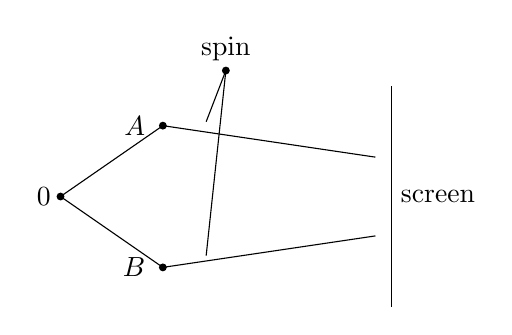
\begin{tikzpicture}[scale=1.0]
\fill (-2,0) circle (0.05);
\node[left] at (-2,0) {$0$};

\fill (-0.7,0.9) circle (0.05);
\node[left] at (-0.8,0.9) {$A$};

\fill (-0.7,-0.9) circle (0.05);
\node[left] at (-0.8,-0.9) {$B$};

\draw (-2,0) -- (-0.7,0.9);
\draw (-2,0) -- (-0.7,-0.9);

\draw (-0.7,0.9) -- (2.0,0.5);
\draw (-0.7,-0.9) -- (2.0,-0.5);

\draw (2.2,-1.4) -- (2.2,1.4);
\node[right] at (2.2,0) {screen};

\fill (0.1,1.6) circle (0.05);
\node[above] at (0.1,1.6) {$\mathrm{spin}$};

\draw (0.1,1.6) -- (-0.15,0.95);
\draw (0.1,1.6) -- (-0.15,-0.75);
\end{tikzpicture}
\caption{Clean schematic of the symmetric detector placement.}
\end{figure}

The recoil example makes the same point less idealized. If the slit plate receives an upward kick when the electron goes through the upper hole and a downward kick when it goes through the lower hole, then the plate itself may store route information. But because the plate is also localized in position, its momentum must already have some quantum uncertainty. If the kick is small compared with that spread, the two recoil states overlap strongly and are not orthogonal. This is precisely where the uncertainty principle enters the discussion. The mark exists only to the extent that the recoil states can be told apart.

The lecture does not write a general environment-overlap formula on the board, but its content is well captured by the cautious reconstruction
\begin{equation}
P_m
=
|\psi_m|^2+|\phi_m|^2
+\psi_m^*\phi_m\langle E_A|E_B\rangle
+\phi_m^*\psi_m\langle E_B|E_A\rangle ,
\end{equation}
where \(|E_A\rangle\) and \(|E_B\rangle\) are the record states left by the two routes. If \(\langle E_A|E_B\rangle=0\), the record is perfectly distinguishing and the interference is gone. If \(\langle E_A|E_B\rangle\) is merely small rather than zero, the fringes are only blurred.

That is how Susskind organizes the later examples. A partial spin kick leaves the detector mostly down with only a little admixture of up, and the pattern is only partially destroyed. Emission of a photon carries route information into the radiation field, but for a slow electron the probability of emission is small and the record is incomplete. A bubble chamber or any track-forming device leaves a far more robust route record, and then the interference is destroyed outright.

One of the lecture's most important clarifications appears here. We do not have to look at the detector. The electron has already done the measurement by becoming entangled with it. It is enough that the information is recorded in principle. We send electrons through one at a time, reset the apparatus, gather statistics on arrival positions, and we see the loss of fringes whether or not anyone ever reads the auxiliary spin.

A second clarification is that the time at which one reads the record is not the essential issue. If a later measurement can reveal which route was taken, then the route information had already been stored in some correlated degree of freedom. That is why Susskind keeps returning to the same rule: ask whether something remembers.

Before leaving this part of the lecture, he briefly generalizes once more. Why do macroscopic objects not visibly spread into fuzzy superpositions? Part of the reason is their mass, but part of it is environmental bombardment. Air, light, and surrounding matter are continually leaving records. The environment is performing measurements all the time.

\section{Measurement Chains, Schr\"odinger's Cat, and the Movable Cut}

From here the lecture scales up the same mechanism. Schr\"odinger's cat is not introduced as a different mystery but as the same entanglement logic with a larger apparatus.

Suppose a gun may or may not fire, and the cat's fate is correlated with the gun. Then the composite system evolves to
\begin{equation}
|\Psi_{\mathrm{cat}}\rangle
=
\alpha\,|{\rm live},{\rm unfired}\rangle
+
\beta\,|{\rm dead},{\rm fired}\rangle .
\end{equation}
What matters is what this is not. It is not an isolated cat state
\[
\alpha\,|{\rm live}\rangle+\beta\,|{\rm dead}\rangle .
\]
The cat is entangled with the gun. The gun has already left a mark, and therefore there are no interference terms between ``live'' and ``dead'' in the ordinary description of the cat. This is, as Susskind emphasizes, the same mathematics as the slit detector.

The same structure persists when Schr\"odinger looks into the box, and when Wigner later asks Schr\"odinger what he saw. Each new observer can be included as another system with a pair of record states. Thus the chain
\[
\text{system} \longrightarrow \text{detector} \longrightarrow \text{observer} \longrightarrow \text{observer of observer}
\]
can be extended as far as we like.

What becomes ambiguous is not the probabilities but the placement of the cut. We may choose to say that the electron's wave function collapsed. Or we may include the detector and say that the combined wave function collapsed. Or we may include Schr\"odinger and postpone the collapse until Wigner's observation. Susskind's point is not that the ambiguity disappears, but that the theory remains consistent. If Wigner asks Schr\"odinger what he saw, the correlations line up.

This also answers an important question about the screen. Why do we talk about the probability that the electron arrives at a given point on the screen? Because the screen is itself another measuring device. A photographic plate blackens, a scintillation screen emits light, or a row of local detectors flips. In each case the arrival position becomes entangled with some macroscopic record. The probability postulate is then applied by constructing the projector onto the relevant subspace and taking its expectation value.

The lecture also sharpens the contrast with classical measurement. In classical physics one imagines that, at least in principle, an experiment can be done gently enough that it does not appreciably disturb the system. In the quantum case that picture fails exactly when incompatible alternatives are at stake. To determine among them, the apparatus must become entangled with the system, and that is a real change of state. Measurement is therefore not just passive observation. It alters whether interference exists.

\section{Entropy, Trace, Density Matrix, and the Next-Lecture Setup}

At this point Susskind says, more or less explicitly, that the lecture has not gone as far as he hoped. He wanted a measure of how entangled two systems are. So he changes gears. The remaining material is preparatory, but it is not an afterthought. It is the exact machinery that will be needed next time.

He begins with the simplest non-entangled example: two spins both up. That is a product state. Looking at one spin tells us nothing new about the other. By contrast, entangled states do correlate subsystems, and the quantity he wants to use to diagnose that correlation is entanglement entropy.

But first we go back to the classical situation.

Suppose a classical system has a finite set of possible states. Entropy, in this discussion, is not merely a property of the system; it is a property of the system together with our knowledge of it. If all we know is that the system lies somewhere בתוך a set of \(n\) equally likely states, then the entropy is
\begin{equation}
S=\log n .
\end{equation}
The logarithm measures, roughly, how many yes-no questions would be needed to pin the state down.

More generally, if the state space carries a probability distribution \(p_i\), then the entropy is
\begin{equation}
S=-\sum_i p_i\log p_i .
\end{equation}
The minus sign is needed because \(\log p_i<0\) whenever \(0<p_i<1\).

The lecture checks that this reproduces the equal-probability case. If
\begin{equation}
p_i=\frac{1}{n}
\qquad \text{for } i\in \mathcal N,
\qquad
p_i=0
\qquad \text{for } i\notin \mathcal N ,
\end{equation}
with \(|\mathcal N|=n\), then
\begin{align}
S
&=
-\sum_i p_i\log p_i \\
&=
-n\left(\frac{1}{n}\right)\log\left(\frac{1}{n}\right) \\
&=
\log n .
\end{align}
The states outside \(\mathcal N\) contribute nothing, because \(p\log p\to 0\) as \(p\to 0\). So the Shannon formula reproduces the simpler \(\log n\) rule exactly where it should.

Susskind then introduces the trace. This is the operation that will play the role of summing over configurations in quantum mechanics.

\begin{definition}
For an operator \(M\) and any complete orthonormal basis \(\{|i\rangle\}\), the trace is
\begin{equation}
\operatorname{Tr}M=\sum_i \langle i|M|i\rangle .
\end{equation}
\end{definition}

A crucial theorem, quoted rather than proved in the lecture, is that the trace is basis independent. If \(M\) happens to be diagonal in some basis, then its diagonal entries are its eigenvalues, and therefore
\begin{equation}
\operatorname{Tr}M=\sum_i \lambda_i .
\end{equation}
This is the sense in which the trace is an invariant.

Now Susskind makes the next step. Suppose someone prepares a system in one of the basis states \(|i\rangle\), but does not tell us which one. We are told only the probabilities \(\rho_i\) for the various preparation outcomes. This is not a coherent superposition. The system is not in \(\rho_1|1\rangle+\rho_2|2\rangle+\cdots\). It is a statistical ensemble of definite preparation states. That is why we need an object more flexible than a state vector.

\begin{figure}[h]
\centering

\includegraphics[width=0.70\textwidth]{lecture_07_figure_06.png}
\caption{Lecture board: schematic transition to a density-matrix description.}
\end{figure}

\begin{figure}[h]
\centering
\begin{tikzpicture}[scale=1.0]
\node at (-2.3,0) {$|\psi\rangle$};
\draw[->] (-1.5,0) -- (-0.3,0);

\draw (1.1,0) circle (1.15);
\fill (0.55,0.45) circle (0.05);
\fill (1.45,0.55) circle (0.05);
\fill (0.75,-0.15) circle (0.05);
\fill (1.55,-0.35) circle (0.05);
\fill (1.05,0.05) circle (0.05);

\node at (1.1,-1.55) {$\rho$};
\end{tikzpicture}
\caption{Clean schematic of the move from a state-vector description to a statistical description.}
\end{figure}

In the basis of preparation states, the density matrix is diagonal:
\begin{equation}
\rho=\mathrm{diag}(\rho_1,\rho_2,\rho_3,\ldots) .
\end{equation}
Its entries are real and nonnegative, and because probabilities sum to one,
\begin{equation}
\operatorname{Tr}\rho=1 .
\end{equation}

Now let \(F\) be an observable. The lecture's central formula is
\begin{equation}
\langle F\rangle=\operatorname{Tr}(F\rho) .
\end{equation}
This is the quantum analog of the classical average \(\sum_i p_i f_i\). To see the analogy, we insert a resolution of the identity,
\begin{equation}
\sum_j |j\rangle\langle j| = I ,
\end{equation}
between \(F\) and \(\rho\). Then
\begin{align}
\langle F\rangle
&=
\operatorname{Tr}(F\rho) \\
&=
\sum_i \langle i|F\rho|i\rangle \\
&=
\sum_{i,j}\langle i|F|j\rangle\langle j|\rho|i\rangle .
\end{align}
If we choose the basis in which \(\rho\) is diagonal, then \(\langle j|\rho|i\rangle\) vanishes unless \(i=j\). Hence
\begin{align}
\langle F\rangle
&=
\sum_i \langle i|F|i\rangle \rho_i \\
&=
\sum_i F_{ii}\rho_i .
\end{align}
This is exactly the weighted average we wanted: the expectation value of \(F\) in each possible preparation state, multiplied by the probability that the system was prepared that way.

The trace also satisfies the cyclic property
\begin{equation}
\operatorname{Tr}(AB)=\operatorname{Tr}(BA) ,
\end{equation}
even when \(A\) and \(B\) do not commute. That is why it does not matter whether we write \(\operatorname{Tr}(F\rho)\) or \(\operatorname{Tr}(\rho F)\).

Finally, Susskind defines the quantum entropy associated with a density matrix:
\begin{equation}
S=-\operatorname{Tr}(\rho\log\rho) .
\end{equation}
If \(\rho\) is diagonal, then \(\log\rho\) is obtained by taking the logarithm of each eigenvalue:
\begin{equation}
\log\rho=\mathrm{diag}(\log\rho_1,\log\rho_2,\log\rho_3,\ldots) .
\end{equation}
So in that basis
\begin{equation}
S=-\sum_i \rho_i\log\rho_i .
\end{equation}
Thus the quantum formula reduces to the classical one when the density matrix is diagonal.

The two limiting cases are exactly those emphasized in the lecture. If one eigenvalue is \(1\) and all the rest are \(0\), then the entropy vanishes. That is the pure-state case. If the density matrix is proportional to the identity, so that all states are equally likely, then the entropy is maximal:
\begin{equation}
\rho \propto I
\qquad \Longrightarrow \qquad
S=\log(\dim \mathcal H) .
\end{equation}

The lecture is very careful here. The entropy of a pure state is zero not because quantum mechanics has somehow ceased to be probabilistic, but because no extra ignorance about preparation remains. The nonzero entropy of a mixed state measures ignorance about which state was prepared.

And now the lecture stops. The payoff is deferred one more step. If a composite system \(AB\) is entangled and we describe only subsystem \(A\), then the right object is a density matrix for \(A\), and that density matrix will carry entropy. If \(A\) and \(B\) are not entangled, it will not. Entanglement entropy itself is therefore not yet computed in this lecture, but every ingredient needed for it has now been assembled.

\section{Summary}

The lecture unfolds in two deliberate movements. First, the discrete two-slit experiment is rebuilt so that we can see exactly where interference comes from and exactly how it disappears when the route becomes entangled with a detector. Measurement is not treated as a vague act of observation but as the establishment of system-apparatus entanglement, with orthogonal record states killing the cross terms. Second, after that mechanism is made precise, Susskind backs up and introduces the mathematics needed to quantify entanglement: classical entropy, the trace, diagonal density matrices, expectation values of the form \(\operatorname{Tr}(F\rho)\), and the quantum entropy \(S=-\operatorname{Tr}(\rho\log\rho)\). The chapter therefore ends at the right place: not with entanglement entropy already in hand, but with the conceptual and mathematical stage set for it.